\documentclass[a4paper, landscape]{article}
\usepackage[a4paper, landscape, margin=1cm]{geometry}
\usepackage{tikz}
\usepackage{amsmath}
\usetikzlibrary{positioning, arrows.meta, shapes.geometric, calc, fit}

\pagestyle{empty}

\tikzset{
    imgnode/.style={rectangle, rounded corners, draw=black!70, fill=brown!20,
                    minimum width=1.7cm, minimum height=1.7cm},
    encoder/.style={rectangle, rounded corners, draw=blue!70, fill=blue!15,
                    minimum width=2.9cm, minimum height=1.5cm, align=center,
                    font=\Large\bfseries},
    latent/.style={font=\LARGE, text=#1!60!black, inner sep=3pt},
    modelbox/.style={rectangle, rounded corners, draw=#1!80, fill=#1!15,
                    minimum width=3.4cm, minimum height=1.6cm, align=center,
                    font=\Large\bfseries},
    regnode/.style={font=\Large\bfseries, text=red!80!black, inner sep=3pt},
    lossarrow/.style={<->, dashed, draw=red!70!black, thick},
    losslabel/.style={font=\Large\bfseries, text=red!70!black},
    loop/.style={rounded corners=4pt}
}

\begin{document}
\begin{center}
\resizebox{\textwidth}{!}{%
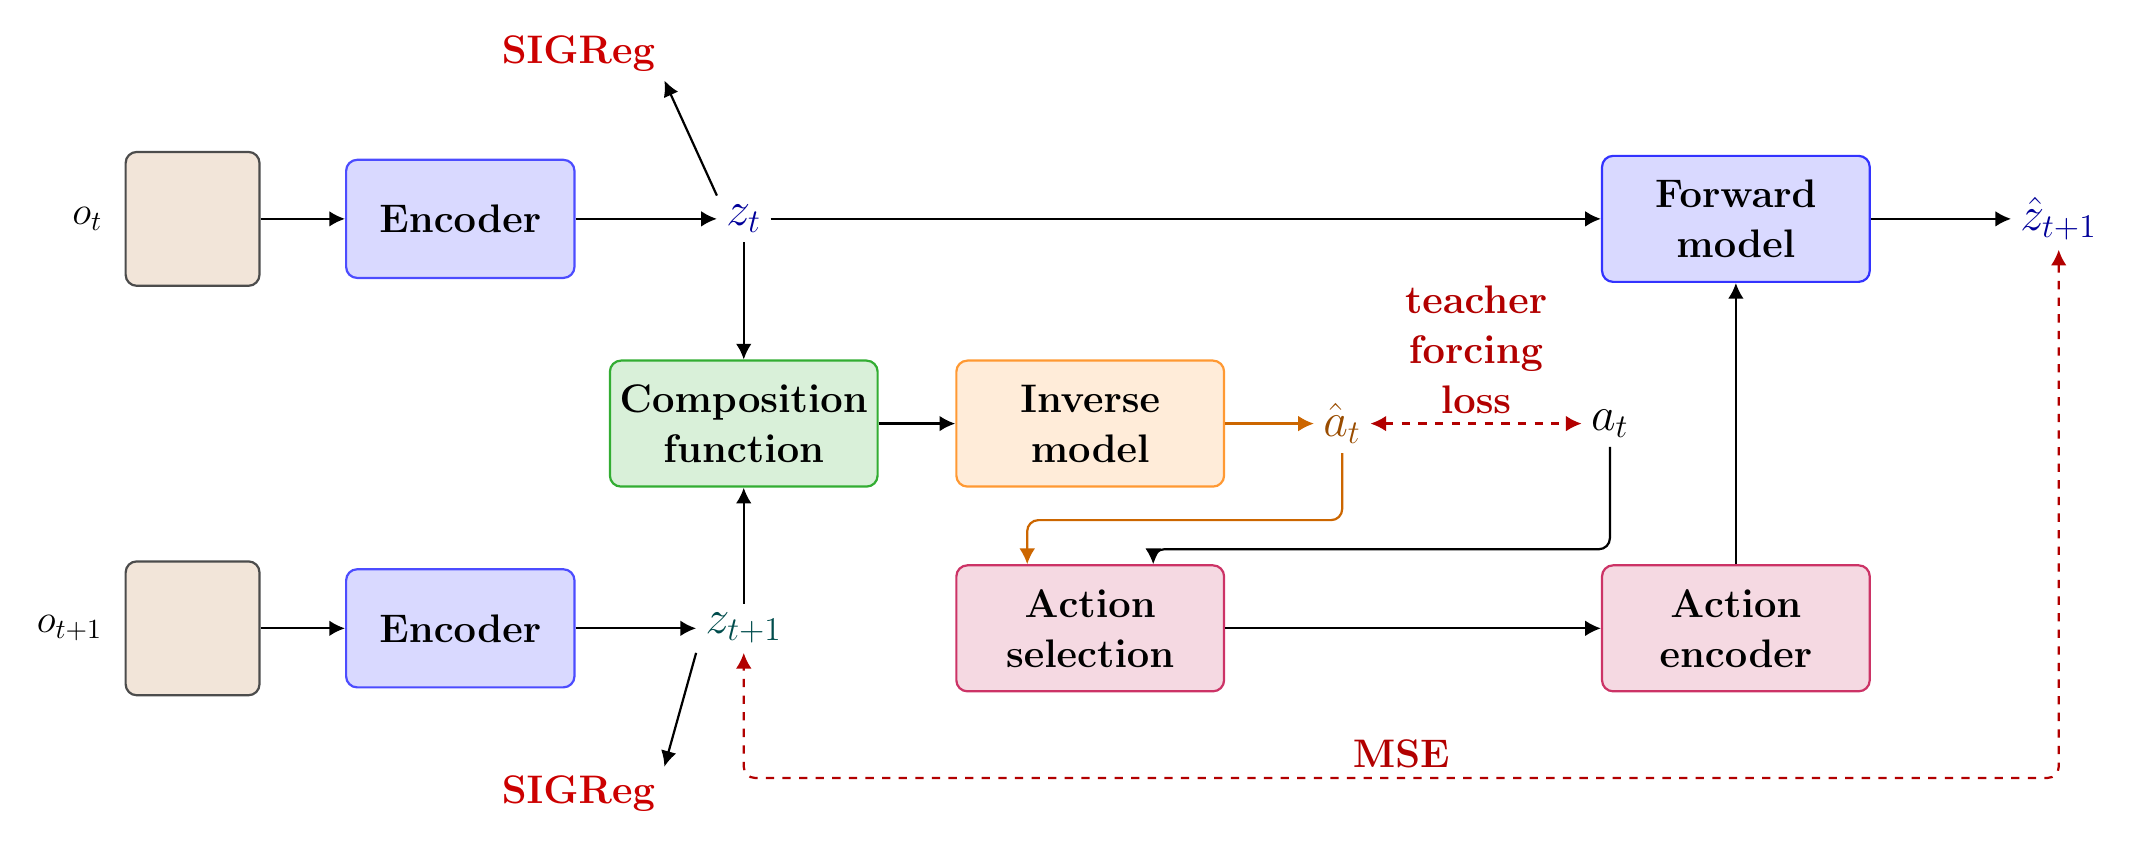
\begin{tikzpicture}[>={Latex[length=2mm, width=2mm]}, thick]

% =====================================================
%  Layout: three horizontal bands, flowing left to right.
%    TOP  (y= 2.6)  o_t   -> Encoder -> z_t  ------> Forward model -> zhat_{t+1}
%    MID  (y= 0.0)  Composition -> Inverse model -> ahat_t  <~~>  a_t
%    BOT  (y=-2.6)  o_t+1 -> Encoder -> z_t+1     Action selection -> Action encoder
%  Natural size is ~27cm x 10cm (aspect ~2.7:1), so at \linewidth the
%  figure is only ~5cm tall. Fonts are deliberately \Large: the picture
%  is scaled by ~0.52, which lands them at roughly 7.5pt on the page.
% =====================================================

% -----------------------------------------------------
% 1. Observations and the shared encoder (two parallel streams)
% -----------------------------------------------------
\node[imgnode] (ot)  at (0, 2.6) {};
\node[left=0.15cm of ot,  font=\Large] {$o_t$};
\node[imgnode] (ot1) at (0,-2.6) {};
\node[left=0.15cm of ot1, font=\Large] {$o_{t+1}$};

\node[encoder] (enc1) at (3.4, 2.6) {Encoder};
\node[encoder] (enc2) at (3.4,-2.6) {Encoder};

\draw[->] (ot.east)  -- (enc1.west);
\draw[->] (ot1.east) -- (enc2.west);

% -----------------------------------------------------
% 2. Latents and SIGReg
% -----------------------------------------------------
\node[latent=blue] (zt)  at (7.0, 2.6) {$z_t$};
\node[latent=teal] (zt1) at (7.0,-2.6) {$z_{t+1}$};

\draw[->] (enc1.east) -- (zt.west);
\draw[->] (enc2.east) -- (zt1.west);

\node[regnode] (sigt)  at (4.9, 4.7) {SIGReg};
\node[regnode] (sigt1) at (4.9,-4.7) {SIGReg};
\draw[->] (zt.north west)  -- (sigt.south east);
\draw[->] (zt1.south west) -- (sigt1.north east);

% -----------------------------------------------------
% 3. Composition function and inverse model
% -----------------------------------------------------
\node[modelbox=green!60!black] (comp) at (7.0,  0) {Composition\\function};
\node[modelbox=orange]         (inv)  at (11.4, 0) {Inverse\\model};

\draw[->] (zt.south)  -- (comp.north);
\draw[->] (zt1.north) -- (comp.south);
\draw[->] (comp.east) -- (inv.west);

% -----------------------------------------------------
% 4. Predicted vs. ground-truth action, and the selector
% -----------------------------------------------------
\node[latent=orange] (ahat) at (14.6, 0) {$\hat{a}_t$};
\node[latent=black]  (at)   at (18.0, 0) {$a_t$};

\draw[->, orange!80!black] (inv.east) -- (ahat.west);
\draw[lossarrow] (ahat.east) -- node[above, losslabel, align=center]
                 {teacher\\forcing\\loss} (at.west);

\node[modelbox=purple] (as)   at (11.4,-2.6) {Action\\selection};
\node[modelbox=purple] (aenc) at (19.6,-2.6) {Action\\encoder};

% the two candidate actions drop into the selector on parallel lanes
\draw[->, loop, orange!80!black]
      (ahat.south) -- ++(0,-0.85) -| ([xshift=-0.8cm]as.north);
\draw[->, loop]
      (at.south)   -- ++(0,-1.30) -| ([xshift=0.8cm]as.north);

\draw[->] (as.east) -- (aenc.west);

% -----------------------------------------------------
% 5. Forward model and the latent prediction loss
% -----------------------------------------------------
\node[modelbox=blue] (fwd)  at (19.6, 2.6) {Forward\\model};
\node[latent=blue]   (zhat) at (23.7, 2.6) {$\hat{z}_{t+1}$};

\draw[->] (aenc.north) -- (fwd.south);
\draw[->] (zt.east)    -- (fwd.west);
\draw[->] (fwd.east)   -- (zhat.west);

% return path for the MSE, routed below every box
\draw[lossarrow, loop] (zhat.south) -- (23.7,-4.5)
      -- node[above, losslabel] {MSE} (7.0,-4.5) -- (zt1.south);

\end{tikzpicture}%
}
\end{center}
\end{document}
